\chapter{Model}
\label{chap:Model}

A very important step in hardware and software development is testing. For an eye tracking system it requires a big effort to do this with real data. The reason for that is that the information where the participant looks at each moment needs to be recorded alongside of the videostreams. For this project real time data processing is needed as there is no hardware available on Gazelle Compute to encode or store the video streams of the cameras.

To optimize the algorithms a simple way of generating new data where the gaze direction and the camera positions are known would simplify the process. 
\section{3D-Modeling Software}
\label{sec:whatIsImportant}

The 3D-Modeling software to create the model needs to fulfill a few requirements:
\begin{itemize}
	\item Correct representation of refracting light
	\item Create animations 
	\item Be scriptable
	\begin{itemize}
		\item Set position and rotation of certain objects at a certain frame
		\item Set camera properties and which camera is active
		\item Read the position and rotation of objects at any frame
	\end{itemize}
	\item (optional)Be free
	\item (optional)Run on Linux
	\begin{itemize}
		\item Server that can be used to render runs Linux containers
	\end{itemize}
	\item (optional)Be easy to learn
\end{itemize}

Blender is able to match all requirements although the last one might be debatable. You can apply a material properties to a surface. This includes refracting. Rotation and position of objects can be inserted as keyframes and it interpolates the steps in-between. 

Blender is also an open source project that is built with Python and has an powerful API that gives access to nearly everything.
\section{Requirements for the Model}
In order to create a flexible model that is close to the reality, the model needs to follow the following requirements:
\begin{itemize}
	\item Correctly represent a human eye
	\item Accommodate for different eye parameters
	\begin{itemize}
		\item Eye diameter
		\item Distance between Eyes
	\end{itemize}
	\item Correctly represent camera placement and rotation
	\item Correctly represent camera properties
	\begin{itemize}
		\item Resolution
		\item Framerate
		\item Field of View
	\end{itemize}
	\item Gaze direction can be animated
	\item Classes rotation and position can be animated
	\item Front facing cameras records gaze direction
\end{itemize}

\section{Human Eye}
A side view of a human eye model is visible in \ref{fig:humanEyeModel}. The camera can only see the front part of the eye. As a result only the cornea, anterior chamber and the iris need to be modeled correctly. The lens can be simplified by a black surface. 

It might be counterintuitive that the cornea extends as much out of the eyeball as visible in \ref{fig:humanEyeModel}. An easy way to verify is to close the eye and move the eyes while holding a finger on the eyelid.
\label{sec:theHumanEye}
\begin{figure}[H]
	\centering
	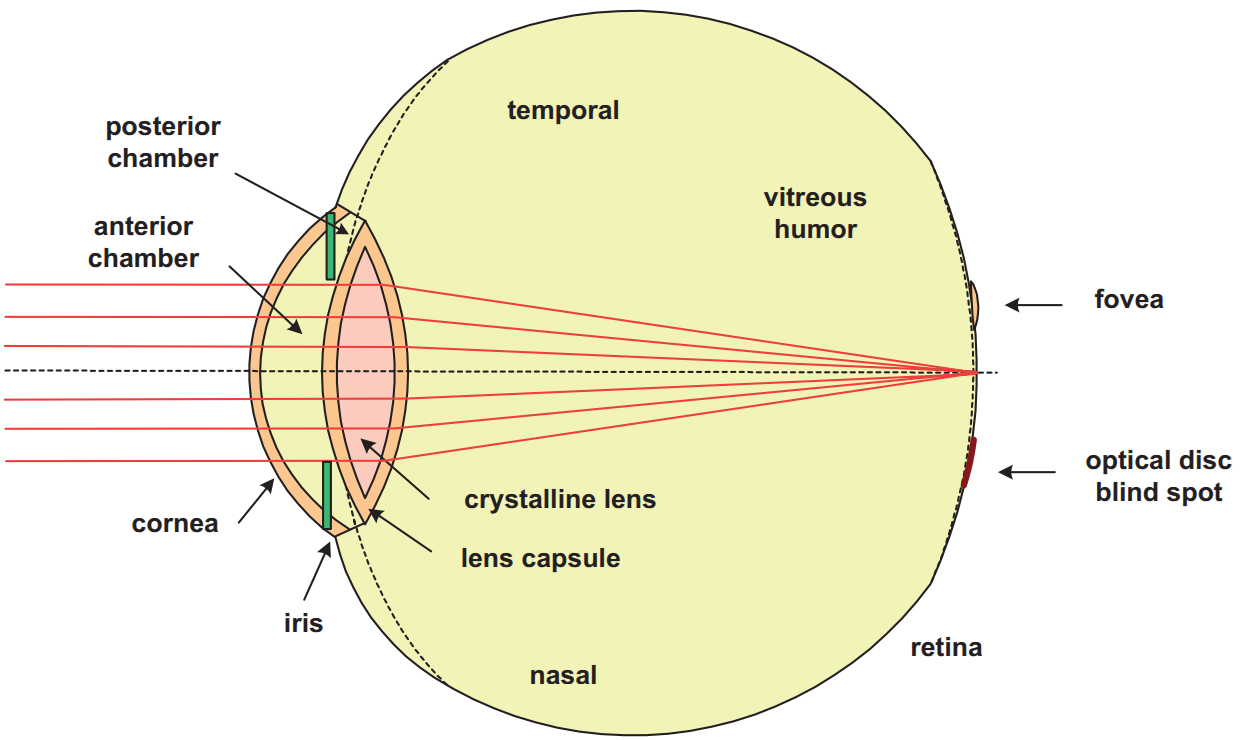
\includegraphics[scale=0.3]{images/human_eye_model.png}
	\caption{Side view of a human eye model \cite{gross:opticalSystems}}
	\label{fig:humanEyeModel}
\end{figure}

There are a few models with different values for the refracting indexes, radii and distances but they are close together in most cases. So the simplified Gullstrand eye was chosen for the model.

\begin{table}[!htb]
\centering
\begin{tabular}{@{}|l|l|l|l|l|l|l|@{}}
	\hline
	\multirow{2}{*}{} & \multicolumn{3}{l|}{\thead{Relaxed}} & \multicolumn{3}{l|}{\thead{Accomodated}} \\ \hhline{~------}
	\thead{ Notaton\\{}} &  \thead{Radius r \\ {}[mm] }        & \thead{Thickness d\\ {}[mm]}    & \thead{Index n\\ {}}        & \thead{Radius r \\ {}[mm] }& \thead{Thickness d \\ {}[mm] }& \thead{Index n\\{} }    \\ \hline
	cornea     &  7.70        & 0.50      & 1.376       &  7.70   &0.50  & 1.376\\ \hline
	anterior chamber & 6.80        & 3.10     & 1.336       & 6.80    & 2.70&1.336 \\ \hline
	crystalline lens     &  10.0    & 3.60          & 1.4085    & 5.33   &   4.0  &  1.426 \\ \hline
	vitreous humor    p  & -6.00      & 17.187         & 1.336    & -5.33  & 13.816  &  1.336  \\ \hline
\end{tabular}
\caption{Properties of the eye with the simplified Gullstrand eye. \cite{gross:opticalSystems}}
\label{tab:gullstrandEye}
\end{table}

A human eye has on average a diameter of 24mm and the distance between the eyes ranges from 56mm to 72mm with the mean for men at 65mm and 62.6mm for women. \cite{gross:opticalSystems}
\section{Base Model}
\label{sec:theModel}

While there are quite a few parameters that need to be adjusted, some will remain the same. Those can be incorporated into a base model that can then be adjusted by a script for each render.

This base model is centred around an accurate eye model that is built with the properties mentioned in section \ref{sec:theHumanEye}. Every eye is a group that can be manipulated with a script as one object. This includes a directed light cone that points where the eye is looking.

An existing model of the glasses is used and placed to approximately represent the position how they would be in the real world. Cutouts for the cameras are used to place them correctly while the rotation is approximated to capture an average positioned eye correctly. The light cones that represent the gaze direction illuminate a small portion of a wall that is captured by the front facing camera and can be seen in figure \ref{fig:base3D}. As with the eye, the cameras and the glasses build a single object that can be moved and rotated. The result can be seen in figure \ref{fig:baseModel} 

\begin{figure}
	\begin{subfigure}{.5\textwidth}
		\centering
		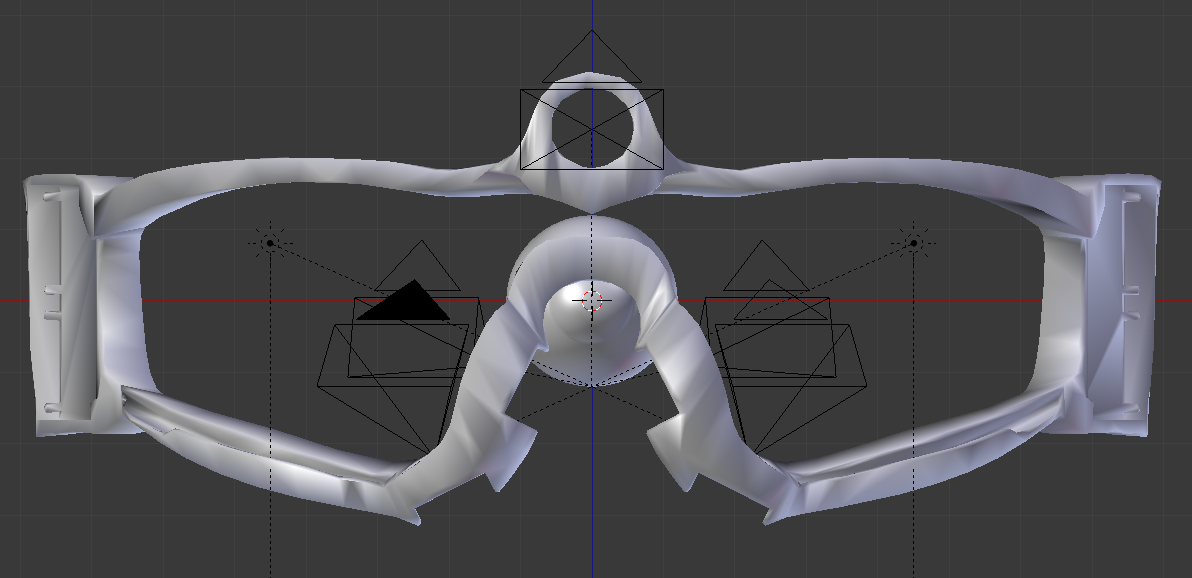
\includegraphics[width=0.9\linewidth]{images/base_model_front.png}
		\caption{Front view of base model}
		\label{fig:baseFront}
	\end{subfigure}
	\begin{subfigure}{.5\textwidth}
		\centering
		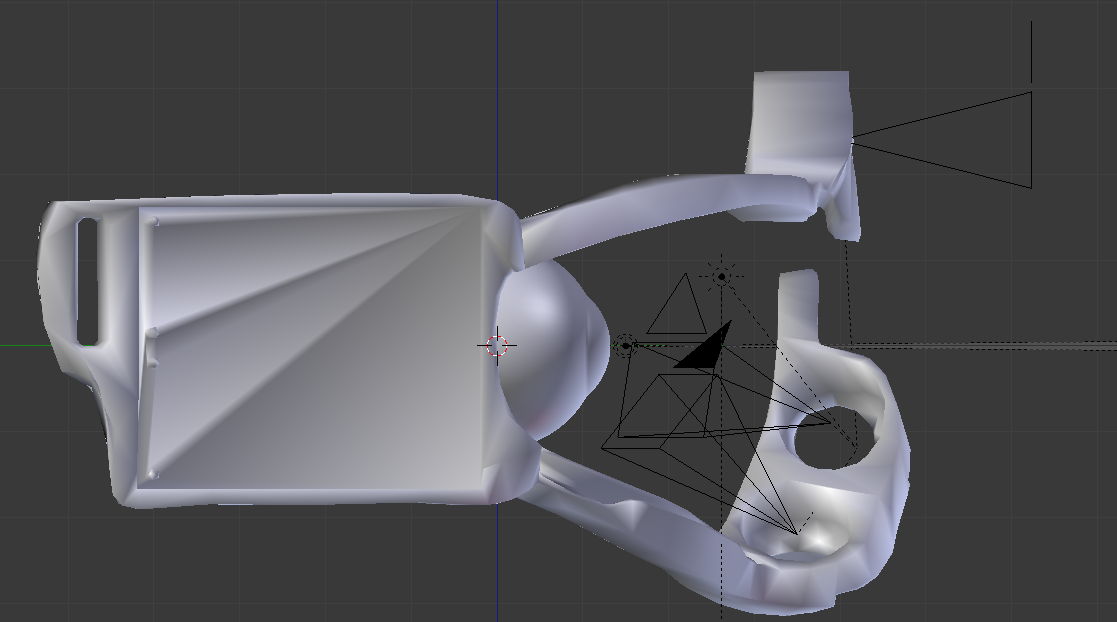
\includegraphics[width=0.787\linewidth]{images/base_model_side.png}
		\caption{Side view of base model}
		\label{fig:baseSide}
	\end{subfigure}
	\begin{subfigure}{.5\textwidth}
		\centering
		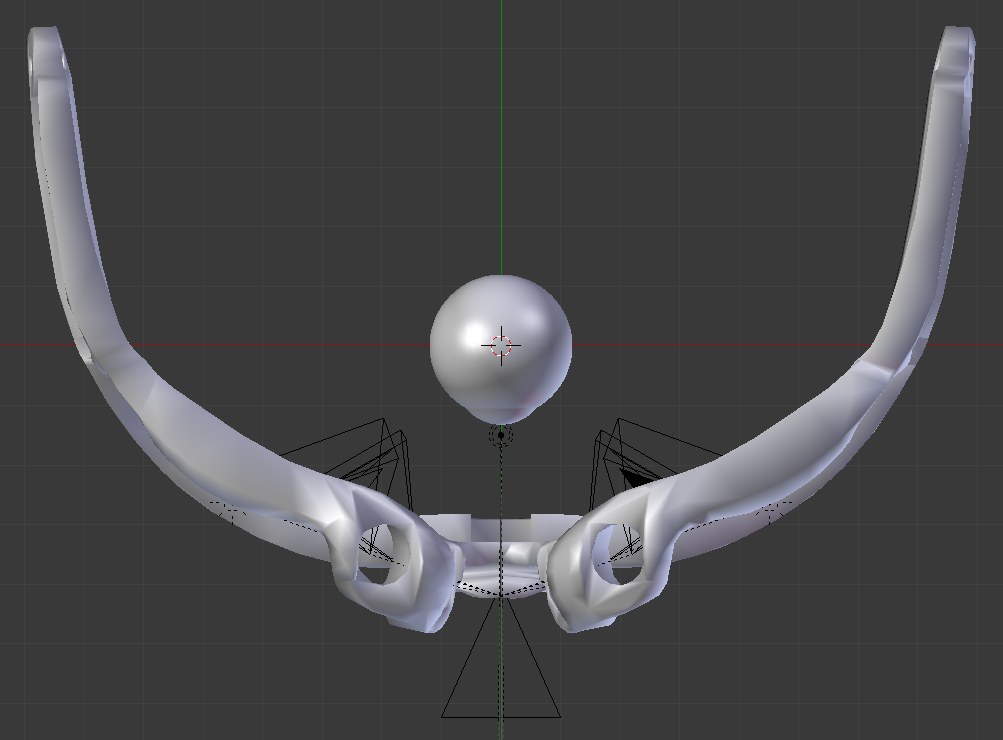
\includegraphics[width=0.9\linewidth]{images/base_model_bottom.png}
		\caption{Bottom view of base model}
		\label{fig:baseBottom}
	\end{subfigure}
	\begin{subfigure}{.5\textwidth}
		\centering
		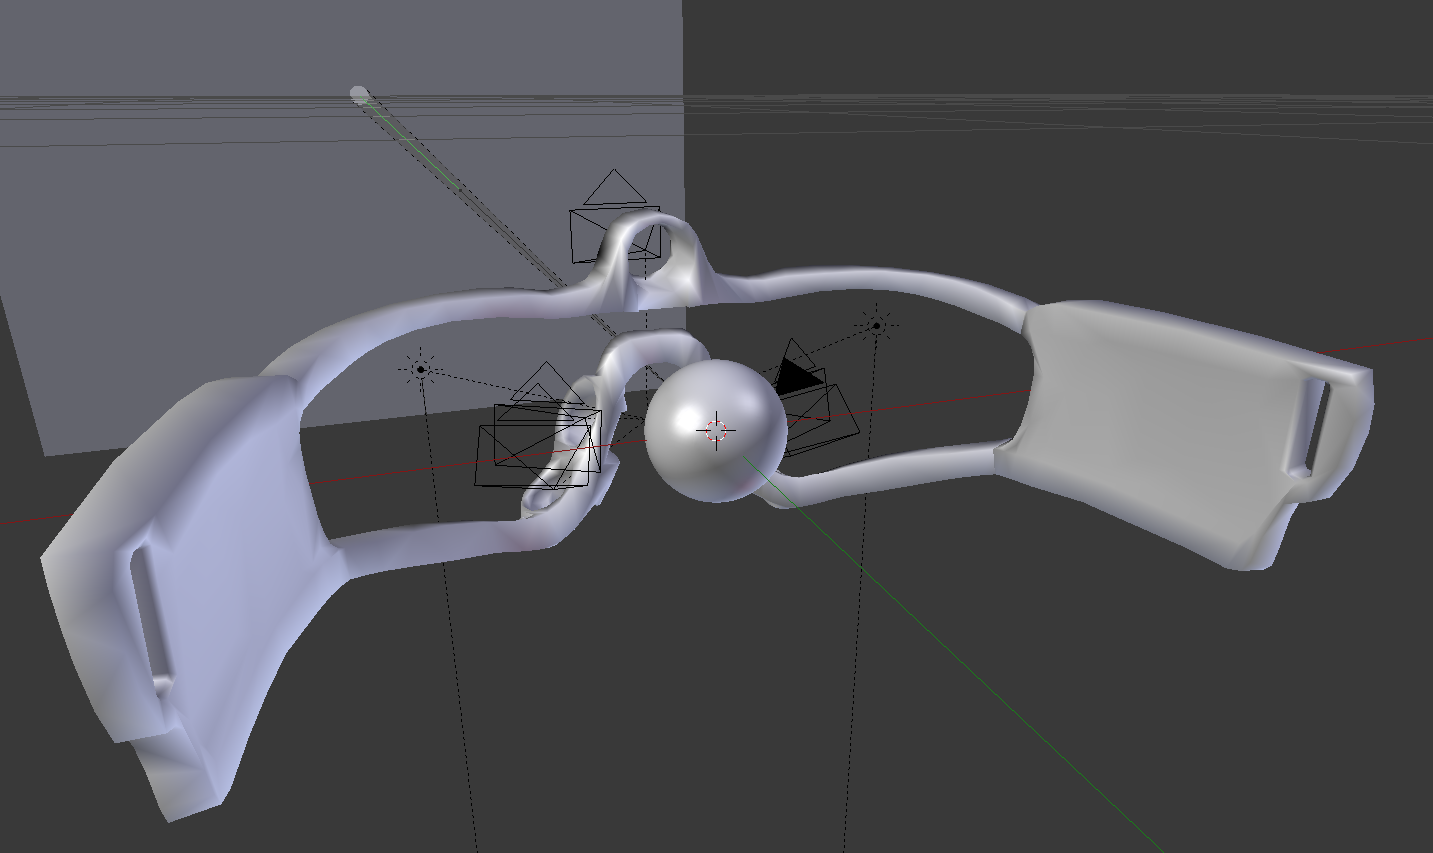
\includegraphics[width=0.9\linewidth]{images/base_model_3D.png}
		\caption{3D-view of base model that shows also the light cone that follows the eye rotation}
		\label{fig:base3D}
	\end{subfigure}
	\caption{Finished base model with eyes in the center. A Script will place the eye correctly and generate an animation from the model that is shown here.}
	\label{fig:baseModel}
\end{figure}
\section{Scripting}
The base model alone is not enough to create meaningful results because there is no animation, the eyes are not placed and blender would just render one camera. Additionally the position and rotation of the eye and glasses needs to be logged for every frame as they are required for comparing the final gaze direction results. To allow a wide variaty of animations to be created a simple way of configuring the script is needed.
\subsubsection{Automate Animation}
This script is written in Python because Blender offers a powerfull Phython API that allows such a script to modify every property in a model. 
JSON is a simple data-interchange format that is easy to read and write for humans. Sites such as \url{http://jsoneditoronline.org/} offer a convenient way to modify JSON. The script uses a JSON file with all the properties as input and adjusts the values in the model and saves a modified blend file for each camera that is ready to be rendered. The properties includes static parameters such as the eye position and diameter and the number of frames that should be rendered. But also dynamic information for keyframes such as the rotation of the eye and position and rotation of the glasses. 
\subsubsection{Automate Process}
With the script the process to generate render output is as follows:
\textbf{}
\begin{lstlisting}
#Use script to generate render ready files
blender base.blend -b -P generate.py -- animation.json
#render the animation for each camera
blender -b leftDown.blend -E CYCLES -t 4 -a
blender -b leftUp.blend -E CYCLES -t 4 -a
blender -b rightDown.blend -E CYCLES -t 4 -a
blender -b rightUp.blend -E CYCLES -t 4 -a
blender -b scene.blend -E CYCLES -t 4 -a
\end{lstlisting}

This is still very time consuming and can be automated further. 

A Makefile offers a convenient way to automate the stages further and make it simple to clean the whole mess up once the generated or rendered files are not needed anymore. 
With the Makefile the whole process is shorter and easier to remember:
\textbf{}
\begin{lstlisting}
#export config file
export ANIMATION_JSON=animation.json
make
make render
\end{lstlisting}

An added benefit is also that make will start the render jobs detached and distribute the available cpu cores equally among the render jobs.